\chapter{$\sigma$-SG($c$)}

To better characterize SG($c$) and TSG we can define a new class of graphs: $\sigma$-SG($c$).

$\sigma$-SG($c$) are unit disk graphs such that the center of the disks belong to $\{(x,y): -\inf < x < \inf, y \in \{0,c\}\}$, so more intuitively we can say that the center of the disks are placed on two parallel horizontal lines.

\section{Characterization of $\sigma$-SG($c$)}

\prop {An $\sigma$-SG($c$) graph $G$ (with $c < 1$) can be characterized by computing $\delta : A \times B \to E$ where $A,B \subseteq G$, $A$ and $B$ are UIG, and $A \cup B = \varnothing$:

\[
    \delta(x,y) =
    \begin{cases}
      xy        & \text{if } \text{dist}(x,y) \leq 1\\
      \varnothing,       & \text{otherwise}
    \end{cases}
\]
}

\proof{ (Idea) Let's take two subsets $A,B \subseteq G$ being $G$ a SG($c$)...  Both of these subsets (A and B are UIG, because each element in each of these subsets is in the same line).

\todo[inline]{Finish proof about characterization -> UIGs}}

\theorem{$\sigma$-SG($\epsilon$) $\subsetneq$ TSG}

\todo[inline]{prove with 2 clique adjacency}

\begin{figure}
\centering

\begin{scaletikzpicturetowidth}{\textwidth}
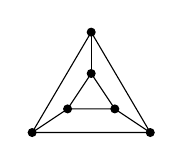
\begin{tikzpicture}[scale=1.5]

%graph
\node[draw,circle,inner sep=1pt,fill,label distance=1cm] (v2) at (0,0.85) {};
\node[draw,circle,inner sep=1pt,fill,label distance=1cm] (v2) at (-0.5,0) {};
\node[draw,circle,inner sep=1pt,fill,label distance=1cm] (v2) at (0.5,0) {};
\draw(0.5,0)--(-0.5,0)--(0,0.85)--(0.5,0);

\node[draw,circle,inner sep=1pt,fill,label distance=1cm] (v2) at (0,0.5) {};
\node[draw,circle,inner sep=1pt,fill,label distance=1cm] (v2) at (0.2,0.2) {};
\node[draw,circle,inner sep=1pt,fill,label distance=1cm] (v2) at (-0.2,0.2) {};
\draw(0,0.5)--(0.2,0.2)--(0.2,0.2)--(-0.2,0.2)--(0,0.5);

\draw(0,0.5)--(0,0.85);
\draw(-0.5,0)--(-0.2,0.2);
\draw(0.2,0.2)--(0.5,0);


\end{tikzpicture}
\end{scaletikzpicturetowidth}

\caption{ Forbidden graph in $\sigma$-SG($\epsilon$) }
\label{fig:forbSigma}
\end{figure}

\proof{By definition, we know that $\sigma$-SG($\epsilon$) $\subset$ TSG because the area where the disks can be placed in $\sigma$-SG($\epsilon$) is included in the area in TSG.

We can prove that $\sigma$-SG($\epsilon$) $\neq$ TSG because we can construct a graph $G$ such that $G \in$ TSG and $G \notin$ $\sigma$-SG($\epsilon$). This graph $F$ is a net$^*$ graph as described in Figure \ref{fig:forbSigma}.
\begin{proofpart}
$F$ is a TSG because we can realize it as a TSG if we take as center of disks $(0,0)$, $(0,z)$, $(0,\epsilon)$, $(1,0)$, $(1,z)$, $(1,\epsilon)$ such that $0 < z < \epsilon$.
\end{proofpart}
\begin{proofpart}
  Now we have to prove that $F$ is a forbidden induced subgraph of $\sigma$-SG($\epsilon$). We will try to construct it by taking a induced subgraph that is representable: we take $F_{-1} = (V,E)$ such that $V(F_{-1}) = V(F)\setminus\{x\}$ with $x\in V(F)$. We notice that $V(F_{-1})$ is $C_{4}$ ($abcd$) with a vertex $e$ attached to two of its vertices (adjacent) creating a triangle $abe$.\\
  The only way to realize this is by taking $a = (0,0)$, $b = (0,\epsilon)$, $c = (1,\epsilon)$, $d = (1,0)$ and $e$
\end{proofpart}

\todo[inline]{How to prove for sigma?}

 }

\todo[inline]{Then in the hierarchy, is MUIG $\subsetneq$ $\sigma$-SG($\epsilon$) or $\subsetneq$ $\sigma$-SG($\epsilon$) true? }
\section{Induced forbidden subgraphs}

\begin{figure}
\centering

\begin{scaletikzpicturetowidth}{\textwidth}
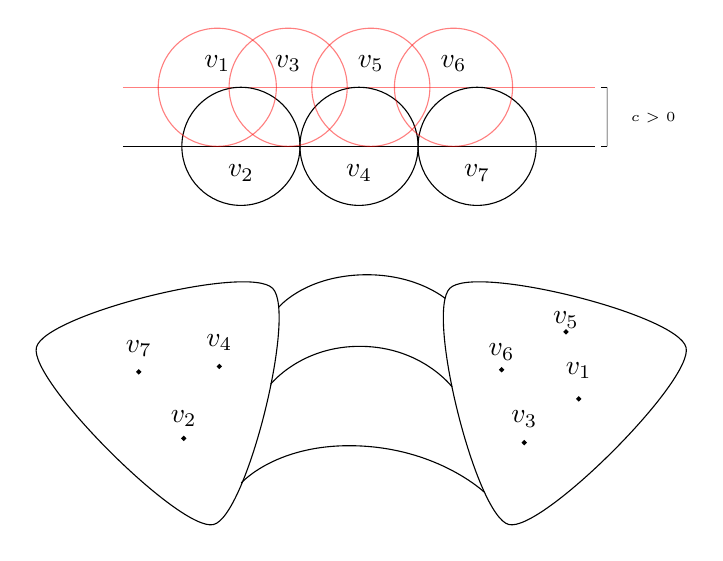
\begin{tikzpicture}[scale=1.5]
\draw (-2,0) -- (2,0);
\draw[red ,opacity = 0.5] (-2,0.5) -- (2,0.5);

\draw  (-1,0) circle [radius=0.5];
\draw[color=black] (-1,-0.2265) node {$v_2$};
\draw  (0,0) circle [radius=0.5];
\draw[color=black] (0,-0.2265) node {$v_4$};
\draw  (1,0) circle [radius=0.5];
\draw[color=black] (1,-0.2265) node {$v_7$};

\draw[red, opacity = 0.5] (0.1,0.5) circle [radius=0.5];
\draw[color=black] (0.1,0.7) node {$v_5$};
\draw[red, opacity = 0.5] (0.8,0.5) circle [radius=0.5];
\draw[color=black] (0.8,0.7) node {$v_6$};
\draw[red, opacity = 0.5] (-0.6,0.5) circle [radius=0.5];
\draw[color=black] (-0.6,0.7) node {$v_3$};
\draw[red, opacity = 0.5] (-1.2,0.5) circle [radius=0.5];
\draw[color=black] (-1.2,0.7) node {$v_1$};
\draw[color=black] (2.4902,0.2393) node {\tiny $c > 0$};

% lines to describe distance (epsilon)
\draw[very thin] (2.1003,0.5) -- (2.1,0);
\draw[very thin] (2.0489,0.5) -- (2.0997,0.5);
\draw[very thin] (2.05,0) -- (2.1,0);



%graph

\draw plot [smooth cycle] coordinates {(-1.2314,-3.2019) (-2.7314,-1.7019) (-0.7314,-1.2019) } ;
\draw plot [smooth cycle] coordinates {(1.2686,-3.2019) (0.7686,-1.2019) (2.7686,-1.7019) } ;


\node[draw,circle,inner sep=0.5pt,fill,label distance=1cm] (v2) at (-1.4847,-2.4724) {};
\draw[color=black] (-1.4847,-2.3019) node {$v_2$};
\node[draw,circle,inner sep=0.5pt,fill,label distance=1cm] (v2) at (-1.1831,-1.8637) {};
\draw[color=black] (-1.1831,-1.6637) node {$v_4$};
\node[draw,circle,inner sep=0.5pt,fill,label distance=1cm] (v2) at (-1.8649,-1.9094) {};
\draw[color=black] (-1.8649,-1.7094) node {$v_7$};

\draw plot [smooth,tension=1.2] coordinates {(-0.6778,-1.3597) (-0.0024,-1.0888)(0.7295,-1.288)} node at (1,0) {};
\draw plot [smooth,tension=1.2] coordinates {(-0.9968,-2.8499) (-0.0099,-2.5359)(1.0588,-2.9266)} node at (1,0){};
\draw plot [smooth,tension=1.2] coordinates {(-0.7488,-2.0147) (0.0223,-1.6933)(0.7878,-2.0368)} node at (1,0){};

\node[draw,circle,inner sep=0.5pt,fill,label distance=1cm] (v2) at (1.86,-2.1379) {};
\draw[color=black] (1.86,-1.8979) node {$v_1$};
\node[draw,circle,inner sep=0.5pt,fill,label distance=1cm] (v2) at (1.399,-2.509) {};
\draw[color=black] (1.399,-2.309) node {$v_3$};
\node[draw,circle,inner sep=0.5pt,fill,label distance=1cm] (v2) at (1.7518,-1.5712) {};
\draw[color=black] (1.7518,-1.4712) node {$v_5$};
\node[draw,circle,inner sep=0.5pt,fill,label distance=1cm] (v2) at (1.2071,-1.8911) {};
\draw[color=black] (1.2071,-1.7411) node {$v_6$};

\end{tikzpicture}
\end{scaletikzpicturetowidth}

\caption{ A representation of a $\sigma$-SG($c$) }
\label{fig:sigma}
\end{figure}

\todo[inline]{Add forbidden subgraphs known for the moment with proofs.}
